\newpage
\def\thoigian{90}%--Thời gian
\de{Đề số 2}{Chương I. Hàm số lượng giác và phương trình lượng giác}
%\ind{PHẦN I.} \inden{Câu trắc nghiệm nhiều phương án lựa chọn. Mỗi câu hỏi học sinh chỉ chọn một phương án.}\\
\begin{center}
	\textbf{PHẦN 1 - CÂU TRẮC NGHIỆM BỐN PHƯƠNG ÁN}
\end{center}
\setcounter{ex}{0}
\Opensolutionfile{ans}[ans/1D1-OTC-Deso1-TN]%--Đặt tên 2D1-Bai1-Dang1-TN
\begin{ex}%[1D1N1-2]
	Số đo theo đơn vị rađian của góc $108^\circ$ là
	\choice
	{\True $\dfrac{3\pi}{5}$}
	{$\dfrac{\pi}{4}$}
	{$\dfrac{3\pi}{2}$}
	{$\dfrac{\pi}{10}$}
	\loigiai
	{
		Ta có $108^\circ= \dfrac{108 \pi}{180}= \dfrac{3\pi}{5}$ (rad). 
	}
\end{ex}
\begin{ex}%[1D1N1-3]
	Cho điểm $M$ trên đường tròn lượng giác như hình vẽ bên. Số đo của góc lượng giác $(OA, OM)$ bằng
	\choice
	{$-\dfrac{\pi}{3}+k \pi$, $k \in \mathbb{Z}$}
	{\True $-\dfrac{\pi}{3}+k 2 \pi$, $k \in \mathbb{Z}$}
	{$-\dfrac{5 \pi}{3}+k 2 \pi$, $k \in \mathbb{Z}$}
	{$\dfrac{5 \pi}{3}+k \pi$, $k \in \mathbb{Z}$}
	\loigiai{
		\begin{center}
			\begin{tikzpicture}[scale=.8,>=stealth, font=\footnotesize, line join=round, line cap=round]
				\draw[fill=black](-2,0) coordinate (A') node[above left] {$A'$} circle (1.5pt) (0,-2) coordinate (B') node[below left] {$B'$} circle (1.5pt) (0,2) coordinate (B) node[above left] {$B$} circle (1.5pt) (0,0) coordinate (O) node[below left]{$O$} circle (1.5pt) (2,0) coordinate (A) node[above right] {$A$} circle (1.5pt) (-60:2) coordinate (M) node [below right] {$M$} circle (1.5 pt) (0.5,0) node[below right] {$\dfrac{\pi}{3}$};
				\draw[very thick] (0,0) circle (2 cm);
				\draw[->] (-3,0)--(3,0) node [below]{$x$};
				\draw[->] (0,-3)--(0,3) node [left]{$y$};
				\clip (-3.5,-3.5) rectangle (3.5,3.5);
				\draw (3,3) node {I} (-3,3) node {II} (-3,-3) node {III} (3,-3) node {IV};
				\draw (M)--(O);
				\pic [draw, angle eccentricity=3] {angle = M--O--A};
				%\draw pic[draw, ->, angle radius=2mm, angle eccentricity=2,"\tiny $125^\circ$"]{angle=A--O--M};
			\end{tikzpicture}
		\end{center}
		Từ hình vẽ ta thấy các góc lượng giác $(OA, OM)$ được tạo bởi tia đầu là tia $OA$, tia cuối là tia $OM$ và quay theo chiều âm một góc $\dfrac{\pi}{3}$ và chỉ có duy nhất một điểm $M$ trên đường tròn lượng giác nên có số đo của các góc lượng giác $(OA, OM) =-\dfrac{\pi}{3} + k2\pi$, $k \in \mathbb{Z}$.
	}
\end{ex}
\begin{ex}%[1D1N2-1]
	Cho góc $-\dfrac{\pi}{2}< \alpha <0$, khẳng định nào sau đây đúng?
	\choice
	{\True $\sin \alpha < 0$}
	{$\cos \alpha < 0$}
	{$\tan \alpha > 0$}
	{$\cot \alpha > 0$}
	\loigiai{
		Ta có $-\dfrac{\pi}{2}< \alpha <0 \Rightarrow \sin \alpha < 0$.
	}
\end{ex}
\begin{ex}%[1D1H2-2]
	Cho góc $\alpha$ thoả mãn $\cos\alpha =-\dfrac{1}{3}$ và $\dfrac{\pi}{2}<\alpha<\pi$. Tính $\sin\alpha$.
	\choice
	{$\sin\alpha=-\dfrac{2\sqrt{2}}{3}$}
	{\True $\sin\alpha=\dfrac{2\sqrt{2}}{3}$}
	{$\sin\alpha=-\dfrac{\sqrt{6}}{3}$}
	{$\sin\alpha=\dfrac{\sqrt{6}}{3}$}
	\loigiai{
		Ta có $\sin^2\alpha=1-\cos^2\alpha=1-\dfrac{1}{9}=\dfrac{8}{9}$.\\
		Suy ra $\sin\alpha =\dfrac{2\sqrt{2}}{3}$ (do $\dfrac{\pi}{2}<\alpha <\pi$ thì $\sin\alpha >0$).
	}
\end{ex}
\begin{ex}%[1D1N3-1]
	Trong các công thức sau, công thức nào \textbf{sai}?
	\choice
	{$\sin 2x=2\sin x\cos x$}
	{\True $\sin 2x=\cos ^2x-\sin ^2x$}
	{$\cos 2x=1-2\sin ^2x$}
	{$\cos 2x=2\cos ^2x-1$}
	\loigiai{
	Ta có	$\cos ^2x-\sin ^2x=\cos 2x$.
	}
\end{ex}
\begin{ex}%[1D1H3-2]
	Đẳng thức nào sau đây là đúng?
	\choice
	{$\sin \left(x-\dfrac{\pi}{6}\right)=\dfrac{\sqrt{3}}{2} \sin x+\dfrac{1}{2} \cos x$}
	{$\sin \left(x-\dfrac{\pi}{6}\right)=\dfrac{1}{2} \sin x-\dfrac{\sqrt{3}}{2} \cos x$}
	{\True $\sin \left(x-\dfrac{\pi}{6}\right)=\dfrac{\sqrt{3}}{2} \sin x-\dfrac{1}{2} \cos x$}
	{$\sin \left(x-\dfrac{\pi}{6}\right)=\dfrac{1}{2} \sin x+\dfrac{\sqrt{3}}{2} \cos x$}
	\loigiai{
		Ta có \begin{align*}
			\sin \left(x-\dfrac{\pi}{6}\right)&=\sin x\cos \dfrac{\pi}{6}-\sin \dfrac{\pi}{6}\cos x\\
			&= \dfrac{\sqrt{3}}{2} \sin x-\dfrac{1}{2} \cos x.
		\end{align*}
	}
\end{ex}
\begin{ex}%[1D1N3-4]
	Trong các khẳng định sau, khẳng định nào đúng?
	\choice
	{\True $\sin a-\sin b=2\cos\dfrac{a+b}{2}\sin\dfrac{a-b}{2}$}
	{$\sin a-\sin b=2\sin\dfrac{a+b}{2}\sin\dfrac{a-b}{2}$}
	{$\sin a-\sin b=2\sin\dfrac{a+b}{2}\cos\dfrac{a-b}{2}$}
	{$\sin a-\sin b=2\cos\dfrac{a+b}{2}\cos\dfrac{a-b}{2}$}
	\loigiai{
		Từ công thức biến đổi tổng thành tích, suy ra $\sin a-\sin b=2\cos\dfrac{a+b}{2}\sin\dfrac{a-b}{2}$.
	}
\end{ex}
\begin{ex}%[1D1N4-4]
	Mệnh đề nào dưới đây là mệnh đề \textbf{sai}?
	\choice
	{Hàm số $y=\sin x$ là hàm số lẻ}
	{\True Hàm số $y=\cos x$ là hàm số lẻ}
	{Hàm số $y=\cot x$ là hàm số lẻ}
	{Hàm số $y=\tan x$ là hàm số lẻ}
	\loigiai
	{
		Mệnh đề \textbf{sai} là \lq\lq Hàm số $y=\cos x$ là hàm số lẻ\rq\rq.
	}
\end{ex}
\begin{ex}%[1D1H4-6]
	Giá trị nhỏ nhất của hàm số $y=2\sin x+5$ là
	\choice
	{\True $3$}
	{$2$}
	{$5$}
	{$4$}
	\loigiai{Ta có $-1\le \sin x\le 1\Leftrightarrow -2+5\le 2\sin x+5\le 2+5\Leftrightarrow 3\le y\le 7$.\\
		Do đó giá trị nhỏ nhất của hàm số $y=2\sin x+5$ là $3$.\\
		Dấu ``='' xảy ra khi $x=-\dfrac{\pi}{2}+k2\pi$, $k\in \mathbb{Z}$.
	}
\end{ex}
\begin{ex}%[1D1N4-7]
	Hình vẽ bên là đồ thị hàm số nào dưới đây
	\begin{center}
		\begin{tikzpicture}[>=stealth,scale=0.77,transform shape] 
			\path
			({-2.5*pi},0) coordinate (X1)
			({-2*pi},0) coordinate (X2)
			({-1.5*pi},0) coordinate (X3)
			({-pi},0) coordinate (X4)
			({-0.5*pi},0) coordinate (X5)
			(0,0) coordinate (O)
			({0.5*pi},0) coordinate (X6)
			({pi},0) coordinate (X7)
			({1.5*pi},0) coordinate (X8)
			({2*pi},0) coordinate (X9)
			({2.5*pi},0) coordinate (X10)
			({-pi},-2) coordinate (A)
			({pi},-2) coordinate (B)
			;
			\draw[->] (-9.5,0) -- (9.5,0) node[below] {\small $x$};
			\draw[->] (0,-1.5) -- (0,1.8) node[right] {\small $y$};
			\draw [dotted] (X2)--({-2*pi},1)--({2*pi},1)--({2*pi},0) (X4)--({-pi},-1)--({pi},-1)--({pi},0) 
			({-pi},0) -- (A) ({pi},0) -- (B);
			\foreach \x/\g/\z in {X1/125/-\tfrac{5\pi}{2},X2/-90/-2\pi,X3/-120/-\tfrac{3\pi}{2},X4/90/-\pi,X5/110/-\tfrac{\pi}{2},X6/-120/\tfrac{\pi}{2},X7/90/\pi,X8/120/\tfrac{3\pi}{2},X9/-90/2\pi,X10/-120/\tfrac{5\pi}{2}} 
			\fill[black] (\x) circle(1pt) +(\g:5mm) node {$\z$};
			\draw [<->] ({-pi},-1.7)--({pi},-1.7) ; 
			\draw (0,0) node[below right]{$O$} (0,-1.7) node[below]{$T=2\pi$}
			(0,1) node[above right]{$1$} (0,-1) node[below right]{$-1$}
			;
			\clip (-9.5,-1.4) rectangle (9.5,1.6) ;
			\draw[thick,samples=100,domain=-9.3:9.3] plot(\x,{cos((\x)*180/pi)});
			
		\end{tikzpicture}
	\end{center}
	\choice
	{$y=\cot x$}
	{\True $y=\cos x$}
	{$y=\sin x$}
	{$y=\tan x$}
	\loigiai{
		Hàm số đồng biến trên mỗi khoảng $(-\pi+k 2 \pi ; k 2 \pi)$ và nghịch biến trên mỗi khoảng $\break(k 2 \pi ; \pi+k 2 \pi)$, $k \in \mathbb{Z}$;
		Có đồ thị là một đường hình sin đối xứng qua trục tung $\Rightarrow y=\cos x$.
	}
\end{ex}
\begin{ex}%[1D1N5-3]
	Phương trình $\sin x=\sin \alpha$ có nghiệm là
	\choice
	{\True $\hoac{&x=\alpha+k 2\pi \\ &x=\pi-\alpha+k 2\pi}$ $(k \in \mathbb{Z})$}
	{$\hoac{&x=\alpha+k \pi \\ &x=\pi-\alpha+k \pi}$ $(k \in \mathbb{Z})$}
	{$\hoac{&x=\alpha+k \pi \\ &x=-\alpha+k \pi}$ $(k \in \mathbb{Z})$}
	{$\hoac{&x=\alpha+k 2\pi \\ &x=-\alpha+k 2\pi}$ $(k \in \mathbb{Z})$}
	\loigiai{
		Ta có $\sin x=\sin \alpha \Leftrightarrow \hoac{&x=\alpha+k2\pi\\&x=\pi-\alpha+k2\pi} (k \in \mathbb{Z})$.
	}
\end{ex}
\begin{ex}%[1D1H5-3]
	Phương trình $\cos x=-\dfrac{\sqrt{3}}{2}$ có tập nghiệm là
	\choice
	{$\left\{\pm \dfrac{\pi}{3}+k\pi; \, k\in \mathbb{Z}\right\}$}
	{$\left\{\pm\dfrac{ \pi}{3}+k2\pi; \, k\in \mathbb{Z}\right\}$}
	{$\left\{\pm \dfrac{\pi}{6}+k\pi; \, k\in \mathbb{Z}\right\}$}
	{\True $\left\{\pm \dfrac{5\pi}{6}+k2\pi; \, k\in \mathbb{Z}\right\}$}
	\loigiai
	{
		Ta có 
		$\cos x = -\dfrac{\sqrt{3}}{2} \Leftrightarrow \cos x = \cos \dfrac{5\pi}{6} \Leftrightarrow x= \pm \dfrac{5\pi}{6}+k2\pi; \, k\in \mathbb{Z}$.
	}
\end{ex}

\Closesolutionfile{ans}

%\ind{PHẦN II.} \inden{Câu trắc nghiệm đúng sai. Trong mỗi ý a), b), c), d) ở mỗi câu, học sinh chọn đúng hoặc sai.}\\
\begin{center}
	\textbf{PHẦN 2 - CÂU TRẮC ĐÚNG SAI}
\end{center}
\setcounter{ex}{0}
\Opensolutionfile{ans}[ans/1D1-OTC-Deso1-DS]%--Đặt tên 2D1-Bai1-DS
\begin{ex}%[1D1N2-2]
	Cho $\cos x=-\dfrac{3}{5}$, với $\dfrac{\pi}{2}<x<\pi$. Khi đó:
	\choiceTF
	{$\cot x=-\dfrac{4}{3}$}
	{$\tan x=-\dfrac{3}{4}$}
	{$\sin x=-\dfrac{4}{5}$}
	{\True $\sin x>0$}
	\loigiai{
		Ta có $\sin^2 x=1-\cos^2 x=1-\left(-\dfrac{3}{5}\right)^2=\dfrac{16}{25}$.\\
		Vì $\dfrac{\pi}{2}<x<\pi$ nên $\sin x=\dfrac{4}{5}$. 
		\begin{itemchoice}
			\itemch Vì $\cot x=\dfrac{\cos x}{\sin x}=-\dfrac{3}{4}$.
			\itemch Vì $\tan x=\dfrac{\sin x}{\cos x}=-\dfrac{4}{3}$.
			\itemch Vì $\sin x=\dfrac{4}{5}$.
			\itemch Vì $\dfrac{\pi}{2}<x<\pi$ nên $\sin x>0$. 
		\end{itemchoice}
	}
\end{ex}
\begin{ex}%[1D1V4-4]
	Cho hàm số $f(x)=\dfrac{10}{3\cos x+5}$.
	\choiceTF
	{\True Hàm số $f(x)$ có tập xác định là tập số thực $\mathbb{R}$}
	{Hàm số $f(x)$ là hàm số lẻ trên $\mathbb{R}$}
	{\True Giá trị lớn nhất của hàm số $f(x)$ trên $\left[-\dfrac{\pi}{2} ; \dfrac{\pi}{2}\right]$ bằng $2$}
	{Nếu $f(x)=3$ thì $\cos 2x=\dfrac{31}{81}$}
	\loigiai{
		\begin{itemchoice}
			\itemch Ta có $3\cos x+5\neq 0$ với mọi $x$.\\
			Vậy hàm số $f(x)$ có tập xác định là tập số thực $\mathbb{R}$.
			\itemch $\forall x\in \mathbb{R}, -x\in\mathbb{R}$, khi đó ta có $f(-x)=\dfrac{10}{3\cos(-x)+5}=\dfrac{10}{3\cos x+5}=f(x)$.\\
			Vậy $f(x)$ là hàm số chẵn.
			\itemch Vì $x\in \left[-\dfrac{\pi}{2} ; \dfrac{\pi}{2}\right]$ nên $ 0\leq\cos x\leq1$ suy ra $ 0\leq3\cos x\leq3$.\\
			Từ đó suy ra $5\leq 3\cos x+5\leq 8$. Do đó $\dfrac{10}{8}\leq f(x)\leq 2$.\\Vậy giá trị lớn nhất của hàm số $f(x)$ trên $\left[-\dfrac{\pi}{2} ; \dfrac{\pi}{2}\right]$ bằng $2$.
			\itemch Ta có 
			\begin{eqnarray*}
				&&f(x)=3\\
				&\Rightarrow& \dfrac{10}{3\cos x+5}=3\\
				&\Rightarrow& 3\cos x+5=\dfrac{10}{3}\\
				&\Rightarrow& \cos x=-\dfrac{5}{9}\\
				&\Rightarrow& \cos 2x=2\cos^{2}x-1=2\cdot\left(-\dfrac{5}{9} \right)^2-1=- \dfrac{31}{81}.
			\end{eqnarray*}
		\end{itemchoice}
	}
\end{ex}

\Closesolutionfile{ans}


%\ind{PHẦN III.} \inden{Câu trắc nghiệm trả lời ngắn}\\
\begin{center}
	\textbf{PHẦN 3 - CÂU TRẮC NGHIỆM TRẢ LỜI NGẮN}
\end{center}
\setcounter{ex}{0}
\Opensolutionfile{ans}[ans/1D1-OTC-Deso1-TLN]%--Đặt tên 2D1-Bai1-DS
\begin{ex}%[1D1V1-6]
	Trong chặng đua nước rút, bánh xe của một vận động viên đua xe đạp quay được $30$ vòng trong $8$ giây. Chọn chiều quay của bánh xe là chiều dương. Xét van $\mathrm{V}$ của bánh xe. Biết rằng bán kính của bánh xe là $35$ cm. Độ dài quãng đường mà vận động viên đua xe đạp đã đi được trong $1$ phút là bao nhiêu mét? (kết quả làm tròn đến hàng đơn vị)
	\shortans[]{495}
	\tikzset{
		ex_markstyle/.style={},
		ex_mark/.style  n args={1}{decoration={ markings, %
				mark= at position 0.5 with
				with{
					\ifnum#1=1
					\draw[ex_markstyle] (0pt,-2pt) -- (0pt,2pt);
					\fi
					\ifnum#1=2
					\draw[ex_markstyle] (-1pt,-2pt) -- (-1pt,2pt);
					\draw[ex_markstyle] (1pt,-2pt) -- (1pt,2pt);
					\fi
					\ifnum#1=3
					\draw[ex_markstyle] (-2pt,-2pt) -- (-2pt,2pt);
					\draw[ex_markstyle] (0pt,-2pt) -- (0pt,2pt);
					\draw[ex_markstyle] (2pt,-2pt) -- (2pt,2pt);
					\fi
					\ifnum#1=4
					\draw[ex_markstyle] (-1pt,-1pt) -- (1pt,1pt);
					\draw[ex_markstyle] (-1pt,1pt) -- (1pt,-1pt);
					\fi
			} },
			pic actions/.append code=\tikzset{postaction=decorate}},
	}
	\definecolor{beige}{rgb}{0.96, 0.96, 0.86}
	\definecolor{frenchblue}{rgb}{0.0, 0.45, 0.73}
	\definecolor{battleshipgrey}{rgb}{0.52, 0.52, 0.51}
	\definecolor{earthyellow}{rgb}{0.88, 0.66, 0.37}
	\begin{center}
		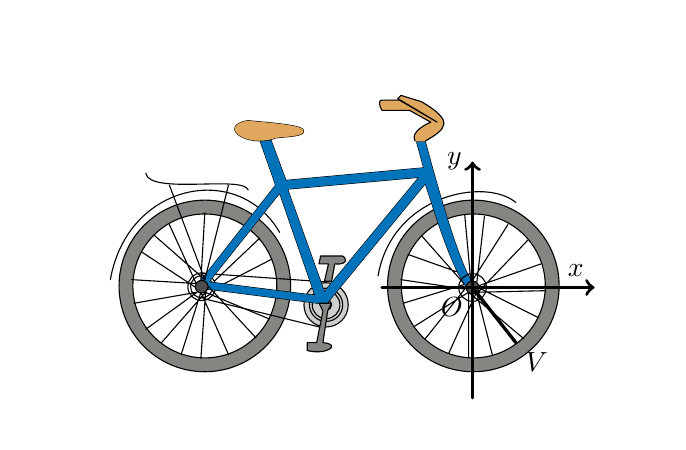
\begin{tikzpicture}[line join=round, line cap=round,scale=1,transform shape]
			\clip (-4,-2.5) rectangle (4,2.5);
			%\draw[gray!] (-3,-4) grid (4,4);
			
			\tikzset{xe_dap/.pic={
					\draw[fill=battleshipgrey] (1.66,-.78) circle (31pt);
					\draw[fill=white] (1.66,-.78) circle (26pt);
					\draw[fill=battleshipgrey] (-1.75,-.78) circle (31pt);
					\draw[fill=white] (-1.75,-.78) circle (26pt);
					\draw[fill=battleshipgrey!40] (-.21,-1.02) circle (8pt);
					\draw (-.21,-1.02) circle (6pt);
					\draw (-.21,-1.02) circle (5pt);
					\draw[fill=battleshipgrey] (-.21,-1.02) circle (2pt);
					
					\draw (-1.79,-.79) circle (5pt);
					\draw (-1.79,-.79) circle (4pt);
					%------------------------------
					\draw (-1.77,-.94)--(-.3,-1.3) (-1.77,-.62)--(-.2,-.73); %xích
					\draw (-0.8,-.1)..controls +(120:1.05) and +(80:1.25) ..(-2.95,-.7)%vành sau
					(0.45,-.65)..controls +(80:1.05) and +(140:.5) ..(2.2,.28)%vành trước
					(-1.2,.44)..controls +(110:.2) and +(-80:.28) ..(-2.5,.65)%yên sau
					;
					\def\S{ 
						(-.91,1.07)--(-.72,.56)--(1.03,.72)--(.94,1.05)--(1.05,1.05)
						..controls +(-75:.3) and +(150:.2) ..(1.68,-.76)--(1.6,-.82)
						..controls +(135:.3) and +(-70:.2) ..(1.05,.52)--(-.2,-1)--(-.27,-.9)--(.97,.6)--(-.7,.45)--(-.18,-1)--(-.315,-1)--(-.8,.4)--(-1.7,-.73
						)--(-.35,-.9)--(-.31,-1)--(-1.87,-.8)--(-.85,.5)--(-1.05,1.07)--cycle
						;}
					\draw[fill=frenchblue] \S;
					\fill[frenchblue] \S;
					
					\def\Y{ 
						(-.5,1.2)
						..controls +(110:.08) and +(-10:.1) ..(-1.2,1.32)
						..controls +(-170:.4) and +(-160:.4) ..(-.85,1.1)
						..controls +(10:.1) and +(-60:.1) ..(-.5,1.2)
						;}
					\draw[fill=earthyellow] \Y;
					\fill[earthyellow] \Y;
					
					\draw (-1.7,-.79)--(-1.1,-1.44) (-1.8,-.86)--(-1.45,-1.65) (-1.74,-.86)--(-1.8,-1.7) (-1.8,-.86)--(-2.05,-1.65) (-1.74,-.86)--(-2.3,-1.5)(-1.85,-.86)--(-2.5,-1.33) (-1.85,-.86)--(-2.65,-1) (-1.85,-.75)--(-2.68,-.7) (-1.88,-.79)--(-2.55,-.35) (-1.86,-.75)--(-2.2,0) (-1.75,-.7)--(-2.4,-0.13) (-1.8,-.7)--(-1.75,.15)(-1.63,-.72)--(-1.05,-.17) (-1.5,-.75)--(-.9,-.44) (-1.77,-.85)--(-.93,-1.2)
					; 
					
					\draw (-1.75,-.7)--(-1.45,.5) (-1.75,-.7)--(-2.2,.5) ; %đỡ yên sau
					
					\draw[fill=battleshipgrey] (-.14,-1)--(-.3,-1)--(-.25,-1.1)--(-.33,-1.5)--(-.45,-1.5)--(-.45,-1.6)..controls +(-15:.25) and +(-5:.25) ..(-.25,-1.5)--(-.19,-1.1)--cycle;%bàn đạp dưới
					
					\draw[fill=battleshipgrey] (-.23,-.72)--(-.18,-.5)--(-.3,-.5)--(-.28,-.4)--(0,-.4)..controls +(-5:.03) and +(-5:.2) ..(-0.1,-.5)--(-.14,-.72)--cycle;%bàn đạp trên
					
					\draw (1.72,-.78)--(2.52,-.5)(1.72,-.86)--(2.35,-.2) (1.72,-.86)--(2.58,-.84)(1.72,-.8)--(2.48,-1.18)(1.6,-.86)--(2.3,-1.45)(1.7,-.86)--(1.9,-1.65)(1.6,-.86)--(1.6,-1.68)(1.7,-.86)--(1.35,-1.63)(1.6,-.76)--(1.05,-1.45)(1.6,-.86)--(.9,-1.3)(1.55,-.76)--(.77,-1)(1.55,-.82)--(.74,-.7)(1.45,-.6)--(.83,-.38)(1.54,-.75)--(1,-.14)(1.63,-.74)--(1.55,.13)(1.63,-.74)--(2.1,0)(1.7,-.77)--(1.8,0.1);
					\draw[fill=black!70] (1.65,-.8) circle (2.3pt);
					\draw (1.65,-.8) circle (5pt);
					\draw[fill=black!70] (-1.79,-.79) circle (2.3pt);
					\draw[fill=earthyellow] 
					(.92,1.06)..controls +(120:.15) and +(-120:0) ..(1.12,1.3)--(.85,1.45)--(.5,1.45)..controls +(120:.15) and +(-120:0) ..(.5,1.58)--(.72,1.58)--(1.2,1.3)--(.7,1.6)--(.74,1.64)--(1,1.56)..controls +(-30:.5) and +(30:.3) ..(1.05,1.06);%vô lăng
			}}
			
			
			\path
			(0,0)pic[scale=1]{xe_dap}
			;
			\def\xmin{0.5} \def\xmax{3.2}
			\def\ymin{-2.2} \def\ymax{.8} 
			\draw[very thick,->] (\xmin,-.8)--(\xmax,-.8) node [above left]{$x$};
			\draw[very thick,->] (1.65,\ymin)--(1.65,\ymax) node [left]{$y$};
			\draw[black,very thick](1.65,-.8)--(2.2,-1.5);
			\node[black] at (2.2,-1.5) [below right]{$V$};
			\node[black] at (1.65,-.8) [below left]{$O$};
			\path 	(2.5,-.9) coordinate (A)
			(2.2,-1.5) coordinate (V)
			(1.65,-.8) coordinate (O)
			;
			
		\end{tikzpicture}
	\end{center}
	\loigiai{Sau $1$ giây, van $\mathrm{V}$ của bánh xe quay được $\dfrac{30}{8}=3{,}75$ (vòng).\\
			Sau $1$ phút, van $\mathrm{V}$ của bánh xe quay được $3{,}75 \cdot 60=225$ (vòng).\\
			Suy ra sau $1$ phút, van $\mathrm{V}$ của bánh xe quay được một góc có số đo là $225\cdot 2\pi=450\pi$.\\
			Mỗi góc ở tâm với sô đo $1$ rad chắn một cung có độ dài bằng bán kính bánh xe $r=0{,}35$ m.\\
			Do đó độ dài quãng đường mà vận động viên đua xe đạp đã đi được trong $1$ phút là $450\pi \cdot 0{,}35\approx 495$ m.
	}
\end{ex}
\begin{ex}%[1D1H5-3]
	Vận tốc của một con lắc đơn $v$ (cm/s) được cho bởi công thức $v(t)=2\sin\left(2t+\dfrac{\pi}{6}\right)$. Lần đầu tiên vận tốc của con lắc đơn bằng $2$ (cm/s) là tại thời điểm $t=\dfrac{\pi}{a}$ (s). Hãy tìm $a$.
	\shortans{$6$}
	\loigiai{
		Ta có
		\begin{eqnarray*}
			& &2\sin\left(2t+\dfrac{\pi}{6}\right) = 2\\
			&\Leftrightarrow& \sin\left(2t+\dfrac{\pi}{6}\right) = 1\\
			&\Leftrightarrow& 2t+\dfrac{\pi}{6}=\dfrac{\pi}{2}+k2\pi\\
			&\Leftrightarrow& t=\dfrac{\pi}{6}+k\pi,\, k\in\mathbb{Z}.
		\end{eqnarray*}
		Lần đầu tiên vận tốc của con lắc đơn bằng $2$ cm/s, ta cần tìm giá trị nhỏ nhất của $t$ lớn hơn $0$. Điều này xảy ra khi $k=0$ hay $t=\dfrac{\pi}{6}$.\\
		Vậy $a=6$.
	}
\end{ex}
\begin{ex}%[1D1V5-6]
	Số giờ có ánh sáng mặt trời của một thành phố A ở vĩ độ $40^\circ$ Bắc trong ngày thứ $t$ của một năm không nhuận được cho bởi hàm số có công thức
	\[d(t)=3\sin \left[\dfrac{\pi}{182} (t-80) \right]+12,\]
	với $t \in \mathbb{Z}$ và $0< t \le 365$. Biết rằng vào một ngày của tháng $6$ dương lịch trong năm đó thì thành phố A có đúng $15$ giờ có ánh sáng mặt trời. Hỏi ngày đó là ngày mấy của tháng $6$?
	\shortans{$20$}
	\loigiai{
		Giả sử thành phố A có đúng $15$ giờ có ánh sáng mặt trời vào ngày thứ $\mathrm{t}_0$.\\
		Ta có $d(t_0)=3 \sin \left[\dfrac{\pi}{182}\left(t_0-80\right)\right]+12$.\\
		Mà $d(t_0)=15$ nên ta có
		\begin{eqnarray*}
			&& 3 \sin \left[\dfrac{\pi}{182}(t_0-80)\right]+12=15 \\
			& \Leftrightarrow& 3 \sin \left[\dfrac{\pi}{182}(t_0-80)\right]=3\\
			& \Leftrightarrow& \sin \left[\dfrac{\pi}{182}(t_0-80)\right]=1\\
			& \Leftrightarrow& \dfrac{\pi}{182}(t_0-80)=\dfrac{\pi}{2}+k2\pi, k \in \mathbb{Z} \\
			& \Leftrightarrow& t_0-80=91+364k, k \in \mathbb{Z} \\
			& \Leftrightarrow& t_0=364k+171, k \in \mathbb{Z}.
		\end{eqnarray*}	
		Mà $0 < t_0 \leq 365 \Leftrightarrow -171 < 364k \leq 194\Leftrightarrow -\dfrac{171}{364} < k \leq \dfrac{97}{182}$.\\
		Mà $k \in \mathbb{Z}$ nên $k=0$ do đó $t_0=171$.\\
		Vậy thành phố A có đúng $15$ giờ có ánh sáng mặt trời vào ngày thứ $171$ trong năm.
		Tức là vào ngày thứ $20$ của tháng $6$ vì tháng 1 (31 ngày), tháng 2 (28 ngày), tháng 3 (31 ngày), tháng 4 (30 ngày), tháng 5 (31 ngày), tháng 6 (20 ngày).
	}
\end{ex}
\begin{ex}%[1D1V4-6]
	Hằng ngày mực nước tại một bến cảng lên xuống theo thủy triều. Độ sâu $h$ (m) của mực nước theo thời gian $t$ (giờ) trong một ngày được cho bởi công thức:
	$$h(t)=11+2\sin\left(\dfrac{\pi}{12}t\right),$$
	với $0\le t\le 24$. Mực nước thấp nhất tại cảng là bao nhiêu?
	\shortans{9}
	\loigiai{
		Với mọi $t$, ta có $-1\le \sin\left(\dfrac{\pi}{12}t\right)\le 1$. Suy ra 
		$$9\le 11+2\sin\left(\dfrac{\pi}{12}t\right) \le 13\Leftrightarrow 9\le h(t)\le 13.$$
		Vậy mực nước thấp nhất tại cảng là $9$ m.
	}
\end{ex}

\Closesolutionfile{ans}

\begin{center}
	\textbf{PHẦN 4 - CÂU TỰ LUẬN}
\end{center}
%\ind{PHẦN IV.} \inden{Tự luận.}\\
\setcounter{ex}{0}
\begin{ex}%[1D1H3-5]
	Cho biết $\cos x=-\dfrac{12}{13}$ và $\pi<x<\dfrac{3 \pi}{2}$. Tính $\cot x$, $\tan 2x$, $\sin \left(\dfrac{\pi}{3}-x\right)$.
	\loigiai{
		Ta có $\pi<x<\dfrac{3 \pi}{2}$ thuộc góc phần tư thứ tư nên $\sin x<0$.\\
		Ta có $\sin^2x=1-\cos^2x=1-\left(-\dfrac{12}{13}\right)^2=\dfrac{25}{169}$, suy ra $\sin x=-\dfrac{5}{13}$.\\
		Do đó $\cot x=\dfrac{\cos x}{\sin x}=-\dfrac{12}{13}:\left(\dfrac{-5}{13}\right)=\dfrac{12}{5}$.\\
		$\tan 2x=\dfrac{\sin 2x}{\cos 2x}=\dfrac{2\sin x\cos x}{2\cos^2x-1}=\dfrac{2\cdot \left(-\dfrac{5}{13}\right)\cdot \left(-\dfrac{12}{13}\right)}{2\left(-\dfrac{12}{13}\right)^2-1}=\dfrac{120}{119}$.\\
		$\sin \left(\dfrac{\pi}{3}-x\right)=\sin \dfrac{\pi}{3}\cos x-\cos \dfrac{\pi}{3}\sin x=\dfrac{\sqrt{3}}{2} \cdot\left(-\dfrac{12}{13}\right)-\dfrac{1}{2} \cdot\left(-\dfrac{5}{13}\right)=\dfrac{5-12 \sqrt{3}}{26}$.
	} 
\end{ex}
\begin{ex}%[1D1V4-2]
	Tìm tập xác định của hàm số $y=\dfrac{\tan 5x}{\sin 4x-\cos 3x}$.
	\loigiai{
		$y=\dfrac{\tan 5x}{\sin 4x-\cos 3x}$.\\
		Ta có $\sin 4x-\cos 3x=\sin 4x-\sin\left(\dfrac{\pi}{2}-3x\right)=2\cos\left(\dfrac{x}{2}+\dfrac{\pi}{4}\right)\cdot\sin\left(\dfrac{7x}{2}-\dfrac{\pi}{4}\right)$.\\
		Điều kiện xác định của hàm số là
		$$\heva{&\cos 5x\ne 0\\&\cos\left(\dfrac{x}{2}+\dfrac{\pi}{4}\right)\neq 0\\&\sin\left(\dfrac{7x}{2}+\dfrac{\pi}{4}\right)\neq 0}\Leftrightarrow \heva{&x\ne \dfrac{\pi}{10}+k\dfrac{\pi}{5} \\&
			x\ne \dfrac{\pi}{2}+k2\pi \\&
			x\ne -\dfrac{\pi}{14}+\dfrac{k2\pi}{7}},k\in\mathbb{Z}.$$
		Vậy tập xác định của hàm số là  $\mathscr{D}=\mathbb{R}\setminus\left\{\dfrac{\pi}{10}+\dfrac{k\pi}{5};\dfrac{\pi}{2}+k2\pi;-\dfrac{\pi}{14}+\dfrac{k2\pi}{7}\Big| k\in \mathbb{Z}\right\}$.
	}
\end{ex}
\begin{ex}%[1D1V5-5]
	Cho phương trình $\cos x = \sin 3x$. Tính tổng các nghiệm thuộc khoảng $(0; 2\pi)$ của phương trình (\textit{làm tròn đến hàng phần chục}).
	\loigiai{
		Ta có
		\begin{align*}
			\cos x = \sin 3x &\Leftrightarrow \cos x = \cos\left(\dfrac{\pi}{2} - 3x\right) \Leftrightarrow \hoac{&x = \dfrac{\pi}{2} - 3x + k2\pi\\&x = -\left(\dfrac{\pi}{2} - 3x\right) + k2\pi}\\
			&\Leftrightarrow \hoac{&4x = \dfrac{\pi}{2} + k2\pi\\&-2x = -\dfrac{\pi}{2} + k2\pi} \Leftrightarrow \hoac{&x = \dfrac{\pi}{8} + k\dfrac{\pi}{2}\\&x = \dfrac{\pi}{4} + k\pi} ,\,  (k \in \mathbb{Z}).
		\end{align*}
		\begin{itemize}
			\item Với $x = \dfrac{\pi}{8} + k\dfrac{\pi}{2}$, ta có $ 0 < \dfrac{\pi}{8} + k\dfrac{\pi}{2} < 2\pi \Leftrightarrow -\dfrac{1}{4} < k < \dfrac{15}{4}$.\\
			Vì $k \in \mathbb{Z}$ nên $k \in \{0; 1; 2; 3\}$. Khi đó, các nghiệm thỏa mãn là
			$$x = \dfrac{\pi}{8};\, x = \dfrac{5\pi}{8}; \, x = \dfrac{9\pi}{8}; \,x = \dfrac{13\pi}{8}.$$
			\item Với $x = \dfrac{\pi}{4} + k\pi$, tương tự ta có các nghiệm thỏa mãn là
			$$x = \dfrac{\pi}{4}; \, x = \dfrac{5\pi}{4}.$$
		\end{itemize}
		Vậy tổng các nghiệm thuộc khoảng $(0; 2\pi)$ của phương trình đã cho là
		$$\dfrac{\pi}{8} + \dfrac{5\pi}{8} + \dfrac{9\pi}{8} + \dfrac{13\pi}{8} + \dfrac{\pi}{4} + \dfrac{5\pi}{4} = \dfrac{28\pi}{8} + \dfrac{6\pi}{4} = \dfrac{7\pi}{2} + \dfrac{3\pi}{2} = 5\pi \approx 15{,}7.$$
	}
\end{ex}